% ============================================================
% Diagram Batang dan Diagram Garis untuk Statistika SMP
% Pendamping artikel: https://pakgun.gezytech.web.id/tikz-diagram-batang-garis-statistika/
% Kompilasi: pdflatex (standalone, butuh paket tikz)
% Data: survei cara berangkat ke sekolah kelas 8C (32 siswa)
%       dan rata-rata UH Matematika kelas 8C (UH1..UH5).
% Ganti frekuensi/labelnya, tinggi batang dihitung dari skala.
% ============================================================
\documentclass[tikz,border=10pt]{standalone}
\begin{document}

% ---------- 1. DIAGRAM BATANG ----------
% Skala: 1 cm = 4 anak ; sumbu frekuensi MULAI DARI NOL.
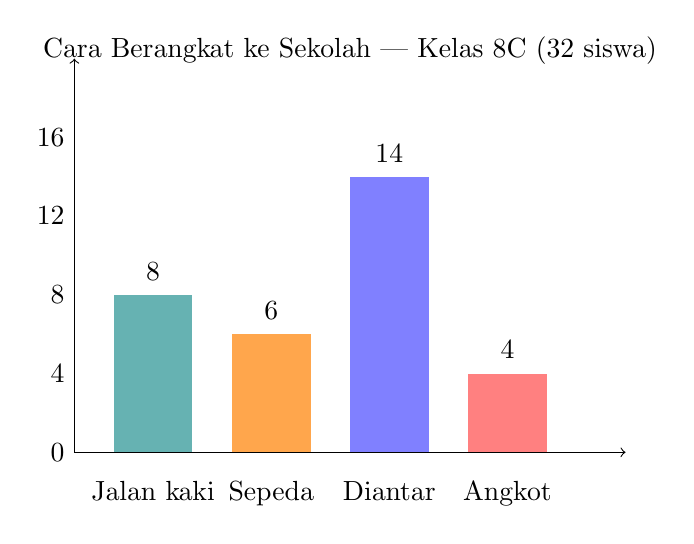
\begin{tikzpicture}
  % sumbu
  \draw[->] (0,0) -- (7,0);   % sumbu kategori
  \draw[->] (0,0) -- (0,5);   % sumbu frekuensi
  % skala sumbu tegak: 1 cm mewakili 4 anak
  \foreach \y/\label in {0/0, 1/4, 2/8, 3/12, 4/16}
    \node[left] at (0,\y) {\label};
  % batang: lebar 1 cm, tinggi = frekuensi / 4 cm
  \fill[teal!60]   (0.5,0) rectangle (1.5,2);    % jalan kaki: 8
  \fill[orange!70] (2,0)   rectangle (3,1.5);    % sepeda: 6
  \fill[blue!50]   (3.5,0) rectangle (4.5,3.5);  % diantar: 14
  \fill[red!50]    (5,0)   rectangle (6,1);      % angkot: 4
  % angka frekuensi di atas batang
  \node at (1,2.3) {8};   \node[below] at (1,-0.25) {Jalan kaki};
  \node at (2.5,1.8) {6}; \node[below] at (2.5,-0.25) {Sepeda};
  \node at (4,3.8) {14};  \node[below] at (4,-0.25) {Diantar};
  \node at (5.5,1.3) {4}; \node[below] at (5.5,-0.25) {Angkot};
  % judul gambar
  \node[above] at (3.5,4.8) {Cara Berangkat ke Sekolah — Kelas 8C (32 siswa)};
\end{tikzpicture}

% ---------- 2. DIAGRAM GARIS ----------
% Sumbu y: 60..90 dengan garis bantu tiap 10 poin.
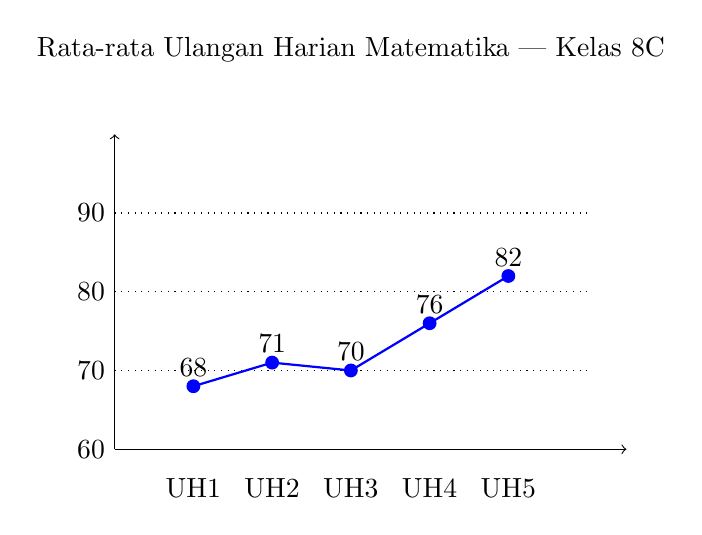
\begin{tikzpicture}
  % sumbu: x = ulangan ke-, y = 60..90
  \draw[->] (0,0) -- (6.5,0);
  \draw[->] (0,0) -- (0,4);
  \foreach \y/\label in {0/60, 1/70, 2/80, 3/90}
    { \draw[dotted] (0,\y) -- (6,\y);
      \node[left] at (0,\y) {\label}; }
  % garis penghubung titik-titik yang BERURUTAN WAKTU
  \draw[thick, blue] (1,0.8) -- (2,1.1) -- (3,1.0)
                     -- (4,1.6) -- (5,2.2);
  % titik data: y = (nilai-60)/10 ; label nilai di atas titik
  \foreach \x/\v in {1/68, 2/71, 3/70, 4/76, 5/82}
    { \fill[blue] (\x,{(\v-60)/10}) circle (2.5pt);
      \node[above] at (\x,{(\v-60)/10}) {\v}; }
  \foreach \x in {1,2,3,4,5}
    \node[below] at (\x,-0.25) {UH\x};
  % judul gambar
  \node[above] at (3,4.8) {Rata-rata Ulangan Harian Matematika — Kelas 8C};
\end{tikzpicture}

\end{document}
